% From mitthesis package
% Version: 1.01, 2023/07/04
% Documentation: https://ctan.org/pkg/mitthesis


\chapter{Patrones de diseño de Gamma}

En este apéndice se resumen los patrones de diseño de Gamma \cite{Gamma:1995:DPE:186897} utilizados en las soluciones a los problemas comunes. En el libro se encuentra una descripción completa de los mismos. Aquí solo se menciona la intención, aplicabilidad, participantes y estructura de cada patrón. El propósito es utilizar este apéndice a manera de complemento al entendimiento de cada aplicación de patrón.

\section{Adapter}

\subsection*{Intención}

Convierte la interfaz de una clase en otra interfaz que los clientes esperan, permitiendo que clases con interfaces incompatibles trabajen juntas. Es una solución para integrar clases existentes sin modificar su código original, asegurando que cumplan con los requisitos de una aplicación específica.

\subsection*{Aplicabilidad}

\begin{itemize}
\item Se desea usar una clase existente cuya interfaz no coincide con la requerida.
\item Se necesita crear una clase reutilizable que coopere con clases no relacionadas o no previstas inicialmente.
\item Se necesita adaptar varias subclases existentes sin modificar su interfaz de manera individual.
\end{itemize}


\subsection*{Participantes}

\begin{itemize}
\item \textbf{Objetivo}\\
Define la interfaz específica del dominio que el cliente utiliza.
\item \textbf{Clientes}\\
Colabora con objetos que cumplen con la interfaz del \textbf{Objetivo}.
\item \textbf{Adaptable}\\
Define una interfaz existente que necesita ser adaptada.
\item \textbf{Adaptador}\\
Adapta la interfaz del \textbf{Adaptable} para que cumpla con la interfaz del \textbf{Objetivo}.
\end{itemize}

\subsection*{Estructura}

\begin{figure}[h]
\caption{Estructura patrón \textbf{Adapter}}
\begin{center}
\begin{tikzpicture}\sf
\umlsimpleclass[x=-4.5,y=1]{Cliente}

\umlclass[x=0,y=1,type=abstract]{Objetivo}
{}
{
\umlvirt{peticion()}
}
\umlclass[below=1.5cm of Objetivo]{Adaptador}
{}
{
peticion()
}
\umlclass[x=6]{Adaptable}
{}
{
peticionConcreta()
}
umluniassoc
\umlinherit[geometry=|-|]{Adaptador}{Objetivo}
\umluniassoc[]{Cliente}{Objetivo}
\umluniassoc[geometry=-|-]{Adaptador}{Adaptable}
\end{tikzpicture}
\end{center}
\end{figure}


\section{Command}


\subsection*{Intención}

El patrón encapsula una solicitud como un módulo, permitiendo parametrizar clientes con diferentes solicitudes, encolar o registrar solicitudes, y admitir operaciones reversibles. Este enfoque facilita la creación de sistemas flexibles y extensibles que manejan comandos de manera uniforme.

\subsection*{Aplicabilidad}

\begin{itemize}
\item Parametrizar objetos con una acción a realizar. Esta parametrización puede expresarse en un lenguaje procedimental mediante una función de \gls{callback}, es decir, una función registrada para ser llamada posteriormente. Los comandos representan una solución orientada a objetos que reemplaza los \glspl{callback}.

\item Especificar, encolar y ejecutar solicitudes en diferentes momentos. Un módulo \textbf{Command} puede tener una vida útil independiente de la solicitud original. Si el receptor de una solicitud puede representarse de forma independiente del espacio de direcciones, puedes transferir un objeto \textbf{Command} a otro proceso y ejecutar la solicitud allí.

\item Soportar la funcionalidad de deshacer (``undo''). El método \textbf{Execute} del \textbf{Command} puede almacenar el estado necesario para revertir sus efectos. La interfaz del \textbf{Command} debe incluir una operación \textbf{Unexecute} para revertir los efectos de una ejecución previa. Los comandos ejecutados se almacenan en una lista de historial, lo que permite deshacer y rehacer a múltiples niveles navegando hacia adelante y hacia atrás en la lista mientras se llaman a \textbf{Unexecute} y \textbf{Execute}.

\item Registrar cambios para que puedan reaplicarse en caso de una falla del sistema. Al ampliar la interfaz del \textbf{Command} con operaciones de carga y almacenamiento, puedes mantener un registro persistente de los cambios. Recuperar un sistema tras una falla implica recargar los comandos registrados desde el disco y reejecutarlos mediante la operación \textbf{Execute}.

\item Estructurar un sistema en torno a operaciones de alto nivel basadas en operaciones primitivas. Esta estructura es común en sistemas de información que admiten transacciones. Una transacción encapsula un conjunto de cambios a los datos. El patrón \textbf{Command} proporciona una forma de modelar transacciones, ya que los comandos tienen una interfaz común, lo que permite invocar todas las transacciones de la misma manera. Además, el patrón facilita la extensión del sistema con nuevas transacciones.
\end{itemize}


\subsection*{Participantes}

\begin{itemize}
\item \textbf{Orden}\\
Declara una interfaz para ejecutar una operación.

\item \textbf{OrdenConcreta}\\
Define una asociación entre un módulo receptor (Receiver) y una acción.
Implementa el método Execute invocando las operaciones correspondientes en el receptor.

\item \textbf{Cliente}\\
Utiliza OrdenConcreta y configura su receptor.

\item \textbf{Invocador}\\
Solicita al comando que lleve a cabo la solicitud.

\item \textbf{Receptor}\\
Conoce cómo realizar las operaciones asociadas con la ejecución de una solicitud. Cualquier clase puede actuar como un receptor.
\end{itemize}


\subsection*{Estructura}

\begin{figure}[h]
\caption{Estructura patrón \textbf{Command}}
\begin{center}
\begin{tikzpicture}\sf
\umlsimpleclass[]{Invocador}
\umlclass[right=2cm of Invocador,type=abstract]{Orden}
{}
{
\umlvirt{ejecutar()}
}
\umlclass[below=2cm of Invocador]{Receptor}
{}
{
acción
}

\umlclass[below=1.45cm of Orden]{OrdenConcreta}
{}
{
ejecutar()
}

\umluniassoc{OrdenConcreta}{Receptor}
\umlinherit{OrdenConcreta}{Orden}
\umluniaggreg{Invocador}{Orden}

\end{tikzpicture}
\end{center}
\end{figure}


\section{State}


\subsection*{Intención}

Permitir que un módulo altere su comportamiento cuando su estado interno cambia. El módulo parecerá cambiar de clase.

\subsection*{Aplicabilidad}

\begin{itemize}
\item El comportamiento de un objeto depende de su estado, y debe cambiar su comportamiento en tiempo de ejecución según ese estado.
\item Las operaciones suelen tener declaraciones condicionales grandes y complejas que dependen del estado del módulo. Este estado generalmente está representado por una o más constantes enumeradas. Frecuentemente, varias operaciones comparten la misma estructura condicional. El patrón separa cada rama de la estructura condicional en una clase independiente. Esto permite tratar el estado del módulo como un módulo por derecho propio, que puede variar independientemente de otros módulos.
\end{itemize}

\subsection*{Participantes}

\begin{itemize}
\item \textbf{Contexto}\\
Define la interfaz de interés para los clientes. Mantiene una instancia de una subclase de EstadoConcreto que define el estado actual.

\item \textbf{Estado}\\
Define una interfaz para encapsular el comportamiento asociado con un estado particular del contexto.

\item \textbf{EstadoConcreto}\\
Cada subclase implementa un comportamiento asociado con un estado del contexto.
\end{itemize}


\subsection*{Estructura}

\begin{figure}[h]
\caption{Estructura patrón \textbf{State}}
\begin{center}
\begin{tikzpicture}\sf
\umlclass[]{Contexto}
{}
{
peticion()
}
\umlnote[below=1cm of Contexto]{Contexto}
{
estado.manejar()
}

\umlclass[right=7cm of Context,type=abstract]{Estado}
{}
{
\umlvirt{manejar()}
}
\umlclass[below left=1.5cm and -0.5cm of Estado]{EstadoConcretoA}
{}
{
manejar()
}
\umlclass[below right=1.5cm and -0.5cm of Estado]{EstadoConcretoB}
{}
{
manejar()
}

\umlinherit[geometry=|-|]{EstadoConcretoB}{Estado}
\umlinherit[geometry=|-|]{EstadoConcretoA}{Estado}
\umluniaggreg[]{Contexto}{Estado}

\end{tikzpicture}
\end{center}
\end{figure}

\section{Mediator}

\subsection*{Intención}
Define un modulo que encapsula cómo interactúa un conjunto de módulos. Fomenta un acoplamiento débil al evitar que los objetos se refieran explícitamente entre sí, y permite variar sus interacciones de manera independiente.

\subsection*{Aplicabilidad}
\begin{itemize}
\item Un conjunto de módulos se comunica de maneras bien definidas pero complejas. Las interdependencias resultantes son desestructuradas y difíciles de comprender.

\item Reutilizar un módulo resulta complicado porque este se refiere y se comunica con muchos otros módulos.

\item Un comportamiento distribuido entre varios módulos debería ser personalizable sin requerir una gran cantidad de subclases.
\end{itemize}

\subsection*{Participantes}

\begin{itemize}
\item \textbf{Mediador} Define una interfaz para comunicarse con los módulos Colega.
\item \textbf{MediadorConcreto} Implementa un comportamiento cooperativo coordinando los módulos Colega. Conoce y mantiene a sus colegas.
\item \textbf{Colega} Conoce a su objeto Mediator y se comunica con se siempre que, de otra forma, se habría comunicado con otro Colega.
\end{itemize}

\subsection*{Estructura}

\begin{figure}[h]
\caption{Estructura patrón \textbf{Mediator}}
\begin{center}
\begin{tikzpicture}\sf
\umlsimpleclass[type=abstract]{Mediador}

\umlsimpleclass[below=1.5cm of Mediador]{MediadorConcreto}

\umlsimpleclass[right=7cm of Mediador,type=abstract]{Colega}

\umlsimpleclass[below left=1.5cm and -0.5cm of Colega]{ColegaConcretoA}

\umlsimpleclass[below right=1.5cm and -0.5cm of Colega]{ColegaConcretoB}

\umlinherit[geometry=|-|]{ColegaConcretoB}{Colega}
\umlinherit[geometry=|-|]{ColegaConcretoA}{Colega}
\umlinherit[]{MediadorConcreto}{Mediador}
\umluniassoc[]{Colega}{Mediador}
\umluniassoc[]{MediadorConcreto}{ColegaConcretoA}
\umluniassoc[geometry=|-|,arm1=-0.7cm,anchor1=-30,anchor2=-150]{MediadorConcreto}{ColegaConcretoB}



\end{tikzpicture}
\end{center}
\end{figure}

\section{Decorator}

\subsection*{Intención}
Agregar responsabilidades adicionales a un objeto de manera dinámica. Los decoradores ofrecen una alternativa flexible a la herencia para extender la funcionalidad.

\subsection*{Aplicabilidad}
\begin{itemize}
\item Agregar responsabilidades a objetos individuales de manera dinámica y transparente, es decir, sin afectar a otros objetos.
\item Para responsabilidades que pueden ser eliminadas.
\item Cuando la extensión mediante herencia es impracticable. A veces, es posible tener una gran cantidad de extensiones independientes, lo que produciría una explosión de subclases para admitir cada combinación. O bien, la definición de una clase puede estar oculta o no estar disponible para la subclase.
\end{itemize}

\subsection*{Participantes}
\begin{itemize}
\item \textbf{Componente} Define la interfaz para módulos a los que se les pueden agregar responsabilidades de manera dinámica.
\item \textbf{ComponenteConcreto} Define un módulo al que se le pueden adjuntar responsabilidades adicionales.
\item \textbf{Decorador} Mantiene una referencia a un módulo \textbf{Componente} y define una interfaz que se ajusta a la interfaz del \textbf{Componente}.
\item \textbf{DecoradorConcreto} Agrega responsabilidades al componente.
\end{itemize}


\subsection*{Estructura}

\begin{figure}[h]
\caption{Estructura patrón \textbf{Decorator}}
\begin{center}
\begin{tikzpicture}\sf
\umlclass[type=abstract]{Componente}{}
{
\umlvirt{operacion()}
}

\umlclass[below left=2cm and -1cm of Componente]{ComponenteConcreto}{}
{
operacion()
}

\umlclass[below right=2cm and -1cm of Componente,type=abstract]{Decorador}{}
{
\umlvirt{operacion()}
}

\umlclass[below right=2cm and -1cm of Decorador]{DecoradorConcretoA}{}
{
operacion() \\
comportamientoAñadido()
}

\umlclass[below left=2cm and -1cm of Decorador]{DecoradorConcretoB}
{
estadoAñadido
}
{
operacion() \\
}

\umlnote[right=4cm of Decorador,width=4.5cm]{Decorador}{
operacion \{\\
\ \ componente.operacion()\\
\}
}

\umlinherit[geometry=|-|]{ComponenteConcreto}{Componente}
\umlinherit[geometry=|-|]{Decorador}{Componente}
\umlinherit[geometry=|-|]{DecoradorConcretoA}{Decorador}
\umlinherit[geometry=|-|,arm1=2.04cm]{DecoradorConcretoB}{Decorador}
\umluniaggreg[geometry=-|-,arm1=3cm,anchor1=20,arg1=componente,pos1=0.5]{Decorador}{Componente}



\end{tikzpicture}
\end{center}
\end{figure}




\section{Proxy}
\label{patronProxy}

\subsection*{Intención}
Proporcionar un sustituto o marcador de posición para otro objeto con el fin de controlar el acceso a este.

\subsection*{Aplicabilidad}

El patrón Proxy es aplicable siempre que se necesite una referencia más versátil o sofisticada a un objeto que un simple puntero. Estas son varias situaciones comunes en las que se puede aplicar el patrón:

\begin{enumerate}
\item Proxy Remoto:

Proporciona un representante local para una instancia en un espacio de direcciones diferente.

\item Proxy Virtual:

Crea instancias costosas bajo demanda.

\item Proxy de Protección:

Controla el acceso a la instancia original.
Es útil cuando las instancias necesitan diferentes derechos de acceso.

\item Referencia Inteligente:

Es un reemplazo para un puntero básico que realiza acciones adicionales cuando se accede a un objeto.
Usos típicos incluyen:
\begin{itemize}
\item Contar el número de referencias a la instancia real para que pueda ser liberado automáticamente cuando no queden más referencias (también llamado punteros inteligentes).
\item Cargar una instancia persistente en memoria cuando se referencia por primera vez.
\item Verificar que la instancia real esté bloqueado antes de acceder a ella, para asegurar que ningún otra instancia pueda modificarlo.
\item 
Este patrón ofrece flexibilidad, seguridad y eficiencia en la gestión de interacciones entre instancias.
\end{itemize}

\end{enumerate}


\subsection*{Participantes}

\begin{itemize}
\item \textbf{Proxy} Mantiene una referencia que permite al proxy acceder al sujeto real. El Proxy puede referirse a un \textbf{Sujuteo} si las interfaces de \textbf{SujetoReal} y \textbf{Sujeto} son las mismas.
Proporciona una interfaz idéntica a la de \textbf{Sujeto}, de manera que un proxy puede ser sustituido por el sujeto real.
Controla el acceso al sujeto real y puede ser responsable de crearlo y eliminarlo.

\item \textbf{Sujeto} Define la interfaz común para \textbf{SujetoReal} y \textbf{Proxy}, de modo que un \textbf{Proxy} se pueda usar en cualquier lugar donde se espere un \textbf{SujetoReal}.

\item \textbf{RealSubject} Define el objeto real que el proxy representa.

\end{itemize}


\subsection*{Estructura}


\begin{figure}[h]
\caption{Estructura patrón \textbf{Proxy}}
\begin{center}
\begin{tikzpicture}\sf
\umlclass[type=abstract]{Sujeto}{}
{
\umlvirt{peticion()}
}

\umlclass[below left=1.5cm and -0.5cm of Sujeto]{SujetoReal}{}
{
peticion() \\
...
}

\umlclass[below right=1.5cm and -0.5cm of Sujeto]{Proxy}{}
{
peticion() \\
...
}

\umlnote[right=2cm of Proxy,width=4cm]{Proxy}{
...\\
sujetoReal.peticion()\\
...}

\umlinherit[geometry=|-|]{SujetoReal}{Sujeto}
\umlinherit[geometry=|-|]{Proxy}{Sujeto}
\umluniassoc[]{Proxy}{SujetoReal}



\end{tikzpicture}
\end{center}
\end{figure}




\section{Iterator}
\label{patronIterator}

\subsection*{Intención}
Proporcionar un modo de acceder secuencialmente a elementos de un módulo sin exponer su representación interna.

\subsection*{Aplicabilidad}

Úsese el patrón Iterador:
\begin{itemize}
\item Para acceder al contenido de un módulo agregado sin exponer su representación interna.
\item Para permitir varios recorridos sobre objetos agregados.
\item Para proporcionar una interfaz uniforme para recorrer diferentes estructuras agregadas (es decir, para permitir la iteración polimórfica).

\end{itemize}


\subsection*{Participantes}

\begin{itemize}
\item \textbf{Iterador} Define una interfaz para recorrer los elementos y acceder a ellos.

\item \textbf{IteradorConcreto} Implementa la interfaz de \textbf{Iterator}.

\item \textbf{Agregado} Define una interfaz para crear una instancia de \textbf{Iterator}.

\item \textbf{AgregadoConcreto} Implementa la interaz de Agregado.

\end{itemize}


\subsection*{Estructura}


\begin{figure}[h]
\caption{Estructura patrón \textbf{Iterador}}
\begin{center}
\begin{tikzpicture}\sf
\umlsimpleclass{Cliente}

\umlclass[left=1.5cm of Cliente]{Agregado}{}
{
crearIterator() \\
}

\umlclass[below=2cm of Agregado]{AgregadoConcreto}{}
{
crearIterator() \\
}


\umlclass[right=1.5cm of Cliente]{Iterador}{}
{
primero() \\
siguiente() \\
haTerminado() \\
elementoActual() \\
}

\umlclass[below right=2cm and 4.83cm of Agregado]{IteradorConcreto}{}
{
primero() \\
siguiente() \\
haTerminado() \\
elementoActual() \\
}

\umlnote[below=1cm of AgregadoConcreto,withd=4cm]{AgregadoConcreto}{
return new IteradorConcreto()
}

\umlinherit{IteradorConcreto}{Iterador}
\umlinherit{AgregadoConcreto}{Agregado}
\umluniassoc[]{Cliente}{Iterador}
\umluniassoc[]{Cliente}{Agregado}


\end{tikzpicture}
\end{center}
\end{figure}









